\documentclass[11pt]{article}

\usepackage{amsmath}
\usepackage{graphicx}
\usepackage{float}
\usepackage{caption}
\usepackage{geometry}
\usepackage{amssymb}
\geometry{margin=1in}
\hyphenpenalty = 10000

\title{CS 736 Assignment \\ Brain MRI Segmentation using FCM and HMRF-GMM-EM}
\author{}
\date{}

\begin{document}

\maketitle

\section{Brain MR Image Segmentation using Modified FCM}

Magnetic Resonance (MR) images often suffer from intensity inhomogeneity (bias field) and noise, which makes segmentation challenging. The goal of this assignment is to segment a brain MR image into three tissue classes:

\begin{itemize}
\item Cerebrospinal Fluid (CSF)
\item Gray Matter (GM)
\item White Matter (WM)
\end{itemize}

A modified Fuzzy C-Means (FCM) algorithm is used which simultaneously estimates the bias field present in the MR image.

The provided dataset contains:

\begin{itemize}
\item A bias-corrupted magnitude MR image
\item A binary mask indicating pixels belonging to the brain
\end{itemize}

Segmentation is performed only on pixels inside the brain mask.

\section{Modified Fuzzy C-Means Formulation}

The corrupted MR image intensity is modeled as

\[
Y_n = b_n c_k + \epsilon_n
\]

where

\begin{itemize}
\item $Y_n$ is the observed intensity
\item $b_n$ is the multiplicative bias field
\item $c_k$ is the class mean of cluster $k$
\item $\epsilon_n$ is noise
\end{itemize}

The algorithm estimates the class means $c_k$, memberships $u_{nk}$ and bias field $b_n$ by minimizing the objective function

\[
J = \sum_n \sum_k u_{nk}^{q}
\sum_{j \in N(n)} w_{nj}(Y_j - b_j c_k)^2
\]

where

\begin{itemize}
\item $q$ is the fuzziness parameter
\item $w_{nj}$ are neighborhood weights
\item $N(n)$ denotes the neighborhood of pixel $n$
\end{itemize}

\section{Algorithm Implementation}

The algorithm iteratively performs the following steps.

\subsection{Update of Class Means}

\[
c_k =
\frac{\sum_n u_{nk}^q \sum_{j \in N(n)} w_{nj} b_j Y_j}
{\sum_n u_{nk}^q \sum_{j \in N(n)} w_{nj} b_j^2}
\]

\subsection{Update of Memberships}

\[
u_{nk} =
\frac{1}{\sum_{l=1}^{K}
\left(\frac{D_{nk}}{D_{nl}}\right)^{\frac{1}{q-1}}}
\]

where

\[
D_{nk} = \sum_{j \in N(n)} w_{nj}(Y_j - b_j c_k)^2
\]

\subsection{Update of Bias Field}

\[
b_n =
\frac{\sum_k u_{nk}^q c_k
\sum_{j \in N(n)} w_{nj} Y_j}
{\sum_k u_{nk}^q c_k^2
\sum_{j \in N(n)} w_{nj}}
\]

To enforce smoothness of the bias field, Gaussian filtering is applied to the estimated bias field after each iteration.

\section{Parameter Selection}

\subsection{Fuzziness Parameter}

The fuzziness parameter was chosen as

\[
q = 1.6
\]

A value greater than 1.5 ensures sufficient fuzziness while maintaining meaningful cluster assignments.

\section{Neighborhood Mask}

A Gaussian neighborhood mask was used to incorporate spatial regularization. The weights were normalized such that

\[
\sum w_{ij} = 1
\]

\begin{figure}[H]
\centering
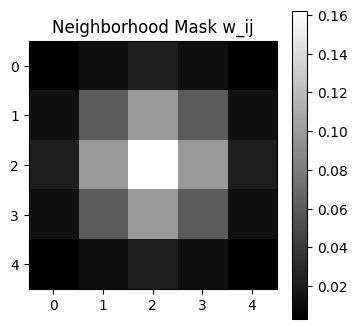
\includegraphics[width=0.35\textwidth]{Q1_gaussian_mask.png}
\caption{Gaussian neighborhood mask used for spatial weighting.}
\end{figure}

\section{Initialization}

\subsection{Initial Membership Estimates}

Membership values were initialized based on intensity ranges within the brain mask. The normalized intensity values were divided into three ranges corresponding to approximate CSF, gray matter, and white matter intensities. Pixels were assigned initial fuzzy memberships based on proximity to these ranges.

\begin{figure}[H]
\centering
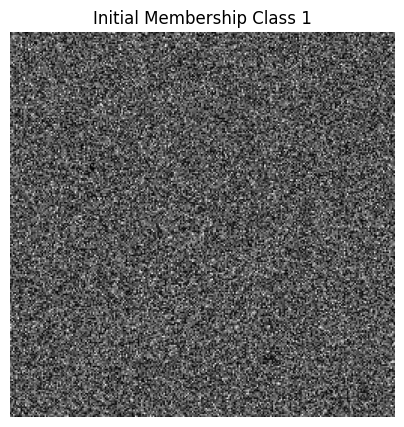
\includegraphics[width=0.3\textwidth]{Q1_init_u1.png}
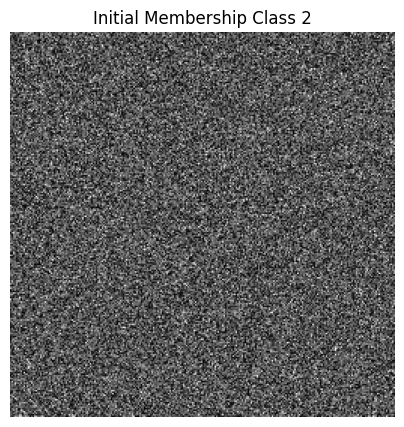
\includegraphics[width=0.3\textwidth]{Q1_init_u2.png}
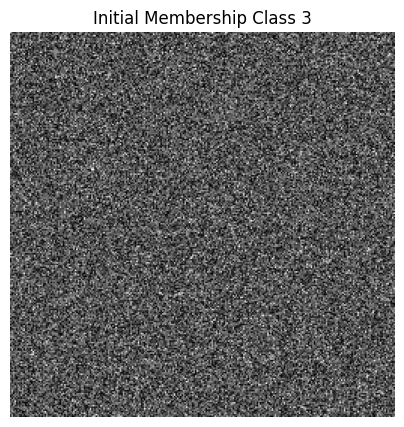
\includegraphics[width=0.3\textwidth]{Q1_init_u3.png}
\caption{Initial membership maps for the three tissue classes.}
\end{figure}

\subsection{Initial Class Means}

Initial class means were chosen from the normalized intensity distribution of the image inside the brain mask.

\[
c = [0.21  0.34 0.44]
\]
\section{Convergence of the Objective Function}

The value of the objective function was computed at every iteration of the modified FCM algorithm. The objective decreases during the early iterations and stabilizes after several iterations, indicating convergence.

\begin{figure}[H]
\centering
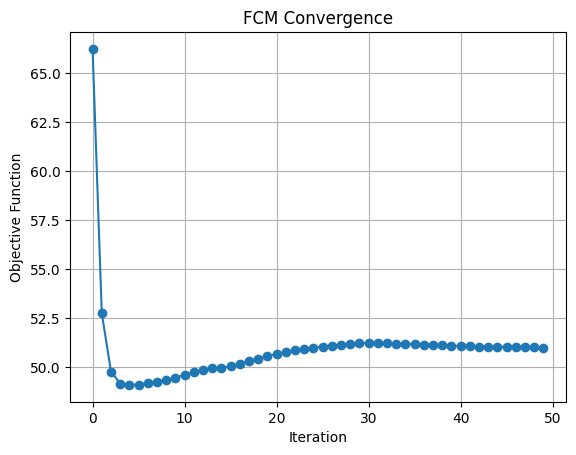
\includegraphics[width=0.6\textwidth]{Q1_FCM_convergence.png}
\caption{Objective function value versus iteration.}
\end{figure}

\section{Segmentation Results}

\subsection{Corrupted MR Image}

\begin{figure}[H]
\centering
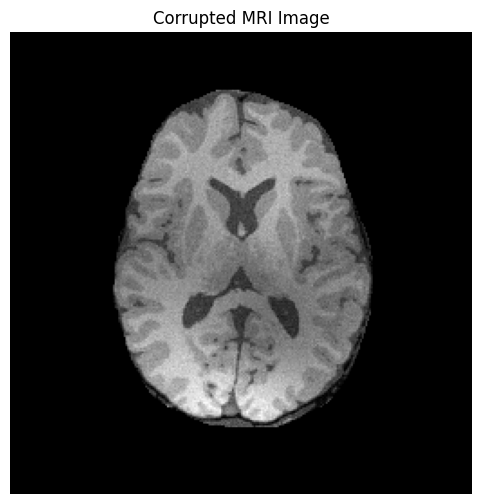
\includegraphics[width=0.45\textwidth]{Q1_corrupted_MRI.png}
\caption{Bias-corrupted MRI image provided in the dataset.}
\end{figure}

\subsection{Optimal Membership Maps}

\begin{figure}[H]
\centering
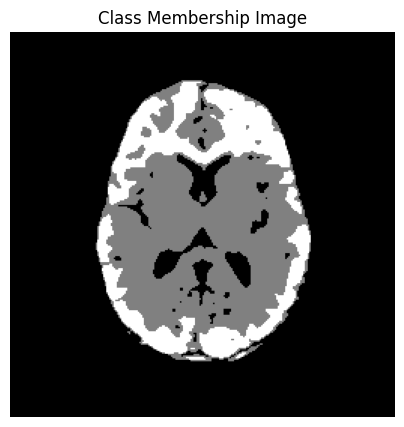
\includegraphics[width=0.3\textwidth]{Q1_class_membership_image.png}
\caption{Estimated membership maps for CSF, Gray Matter and White Matter.}
\end{figure}

\subsection{Estimated Bias Field}

\begin{figure}[H]
\centering
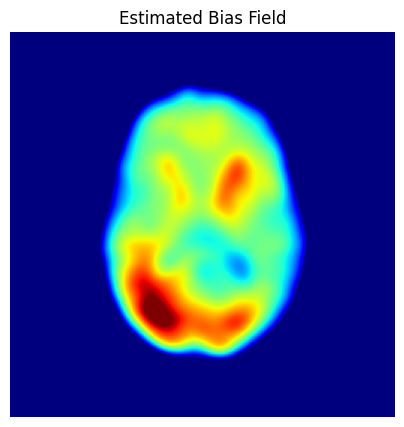
\includegraphics[width=0.45\textwidth]{Q1_bias_field.png}
\caption{Estimated bias field.}
\end{figure}

\subsection{Bias Removed Image}

The bias removed image is computed as

\[
A_n = \sum_k u_{nk} c_k
\]

\begin{figure}[H]
\centering
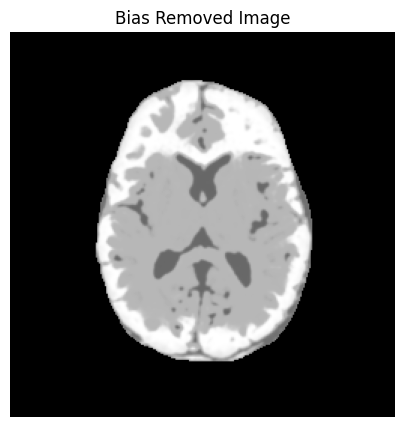
\includegraphics[width=0.45\textwidth]{Q1_bias_removed_image.png}
\caption{Bias removed MRI image.}
\end{figure}

\subsection{Residual Image}

The residual image is computed as

\[
R_n = Y_n - A_n b_n
\]

\begin{figure}[H]
\centering
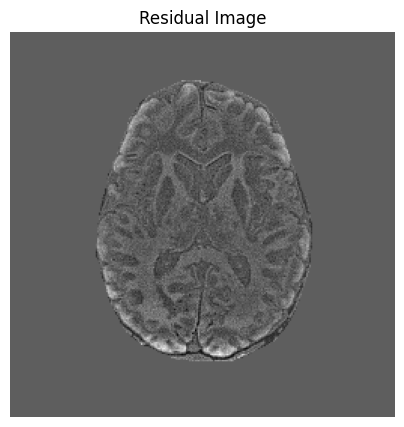
\includegraphics[width=0.45\textwidth]{Q1_residual_image.png}
\caption{Residual image.}
\end{figure}

\section{Optimal Class Means}

The final estimated class means obtained from the algorithm are

\[
c = [0.1769, \; 0.3124, \; 0.4367]
\]

These correspond to the expected ordering of brain tissue intensities:

\begin{itemize}
\item CSF (lowest intensity)
\item Gray Matter (intermediate intensity)
\item White Matter (highest intensity)
\end{itemize}

\section{Uniqueness of the Solution}

The optimization problem does not have a unique solution due to scale ambiguity between the bias field and class means.

From the model

\[
Y_n = b_n c_k
\]

if

\[
c_k' = \alpha c_k
\]

and

\[
b_n' = \frac{b_n}{\alpha}
\]

then

\[
b_n' c_k' = b_n c_k
\]

and the reconstructed image remains unchanged. Therefore the solution is not unique.

\subsection{Ensuring a Unique Solution}

To remove this ambiguity, the bias field was normalized after each iteration so that the average bias inside the brain equals 1:

\[
b_n \leftarrow \frac{b_n}{\text{mean}(b_n)}
\]

\subsection{Implementation}

The following normalization step was implemented in the code:

\begin{verbatim}
b = b / mean(b[mask])
\end{verbatim}

This removes the scale ambiguity and ensures a unique solution.

\section{Conclusion}

The modified FCM algorithm successfully segmented the brain MR image into three tissue classes while simultaneously estimating the bias field. The estimated class means correspond to the expected ordering of CSF, gray matter, and white matter intensities. The estimated bias field is smooth and consistent with typical MRI intensity inhomogeneity patterns. The algorithm converged after several iterations, demonstrating the effectiveness of incorporating spatial regularization and bias estimation within the FCM framework.

\newpage
\section{Brain MRI Segmentation using EM with GMM and MRF}

\subsection{Problem Description}

In this part, the brain MRI image is segmented into three tissue classes (CSF, Gray Matter, White Matter) using an Expectation-Maximization (EM) framework with:

\begin{itemize}
\item Gaussian Mixture Model (GMM) for intensity modeling
\item Markov Random Field (MRF) prior for spatial regularization
\end{itemize}

This approach improves segmentation by incorporating both intensity and spatial information.

\subsection{Model Formulation}

Let:

\begin{itemize}
\item $Y = \{Y_n\}$ be observed intensities
\item $X = \{X_n\}$ be hidden labels
\item $K = 3$ classes
\end{itemize}

Each class is modeled using a Gaussian distribution:

\[
P(Y_n | X_n = k) = \mathcal{N}(Y_n; \mu_k, \sigma_k^2)
\]

\subsection{MRF Prior}

A Potts model is used for spatial smoothness:

\[
P(X) \propto \exp(-\beta U(X))
\]

where

\[
U(X) = \sum_{(n,m) \in \mathcal{N}} \mathbb{I}(X_n \neq X_m)
\]

The parameter $\beta$ controls the strength of spatial regularization.


\subsection{Algorithm}

The algorithm alternates between the following steps:

\subsubsection{Initialization}

K-means clustering is applied to the intensities inside the brain mask to obtain:

\begin{itemize}
\item Initial class means $\mu_k$
\item Initial variances $\sigma_k^2$
\item Initial labels
\end{itemize}


\subsubsection{E-Step (Mean-Field Approximation)}

The posterior membership probabilities are computed as:

\[
r_{nk} \propto \mathcal{N}(Y_n | \mu_k, \sigma_k^2) \cdot \exp\left(\beta \sum_{j \in \mathcal{N}(n)} r_{jk}\right)
\]

This incorporates both:

\begin{itemize}
\item GMM likelihood
\item MRF spatial prior using neighboring memberships
\end{itemize}


\subsubsection{M-Step}

The parameters are updated as:

\[
\mu_k = \frac{\sum_n r_{nk} Y_n}{\sum_n r_{nk}}
\]

\[
\sigma_k^2 = \frac{\sum_n r_{nk}(Y_n - \mu_k)^2}{\sum_n r_{nk}}
\]


\subsubsection{Label Update (Modified ICM)}

Labels are updated using:

\[
X_n = \arg\max_k \left[
\log P(Y_n | k) + \beta \cdot \text{neighbor count}_k
\right]
\]

The update is accepted only if the global posterior increases.


\subsection{Parameter Selection}

\[
K = 3, \quad \beta = 1.0
\]

The value of $\beta$ was chosen to balance:

\begin{itemize}
\item Noise reduction
\item Preservation of boundaries
\end{itemize}


\subsection{Convergence Behavior}

The log-posterior was tracked across iterations and was observed to increase monotonically, indicating convergence. The algorithm typically converged after 10-15 iterations.

\subsection{Results}

\subsubsection{Corrupted MRI Image}

\begin{figure}[H]
\centering
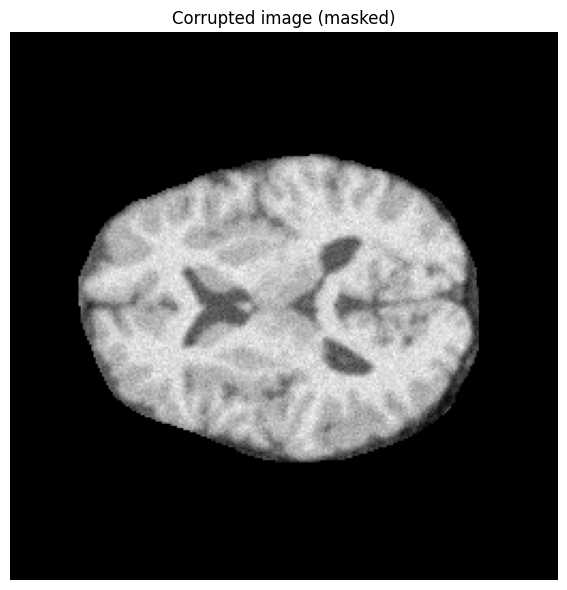
\includegraphics[width=0.45\textwidth]{Q2_corrupted_MRI.png}
\caption{Input MRI image.}
\end{figure}


\subsubsection{Segmentation with MRF ($\beta = 1.0$)}

\begin{figure}[H]
\centering
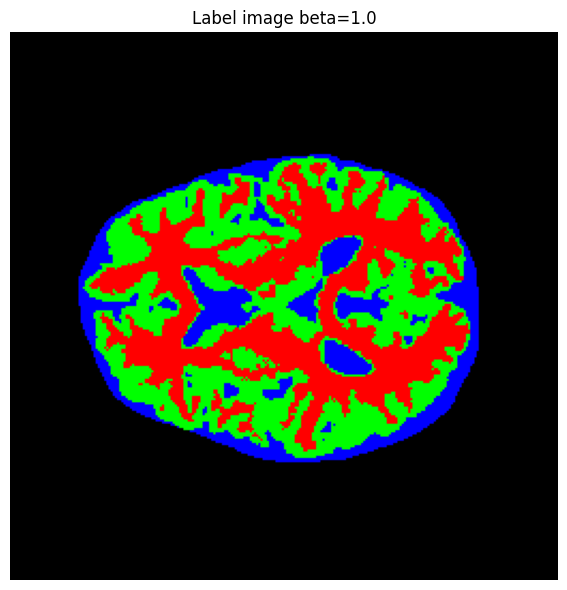
\includegraphics[width=0.45\textwidth]{Q2_segmented_output_beta_1.png}
\caption{Segmentation with MRF prior.}
\end{figure}


\subsubsection{Segmentation without MRF ($\beta = 0$)}

\begin{figure}[H]
\centering
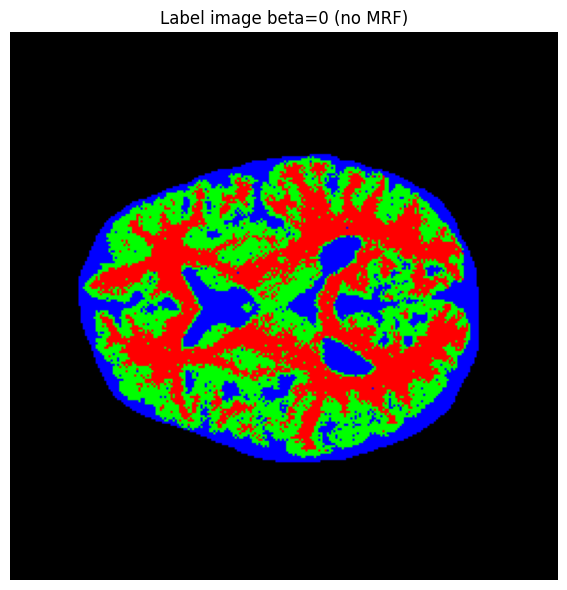
\includegraphics[width=0.45\textwidth]{Q2_segmented_output_beta_0.png}
\caption{Segmentation without MRF prior.}
\end{figure}


\subsubsection{Membership Maps (with MRF)}

\begin{figure}[H]
\centering
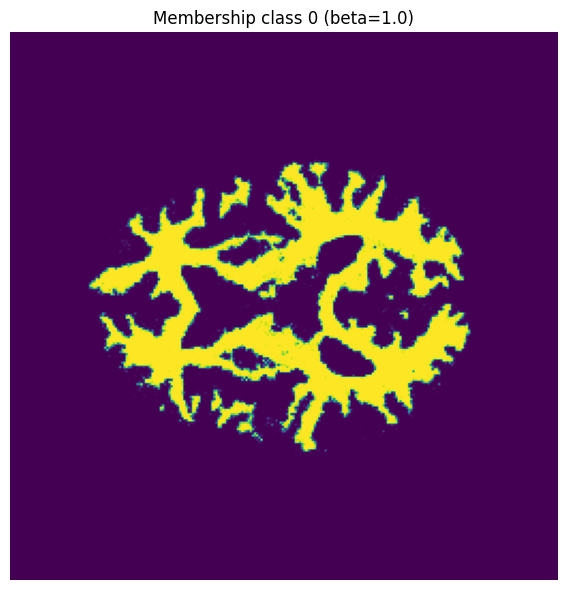
\includegraphics[width=0.3\textwidth]{Q2_membership_class_0_beta_1.png}
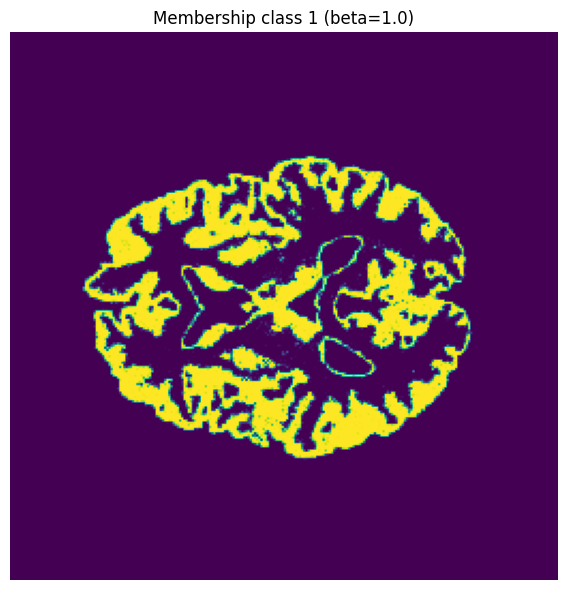
\includegraphics[width=0.3\textwidth]{Q2_membership_class_1_beta_1.png}
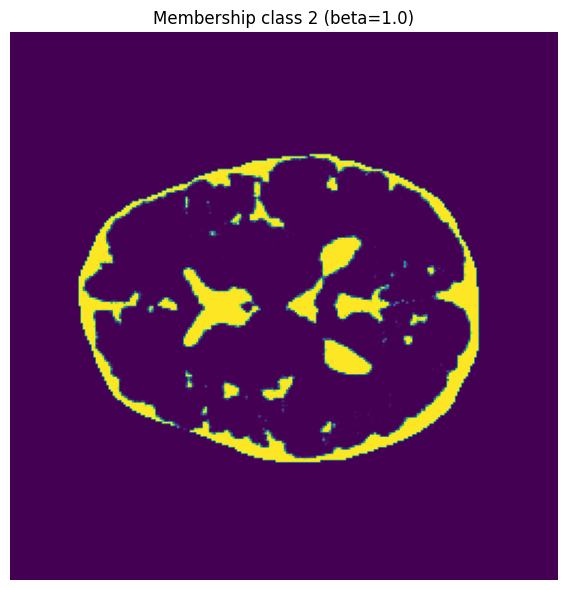
\includegraphics[width=0.3\textwidth]{Q2_membership_class_2_beta_1.png}
\caption{Membership maps for the three classes.}
\end{figure}

\subsubsection{Membership Maps (without MRF)}

\begin{figure}[H]
\centering
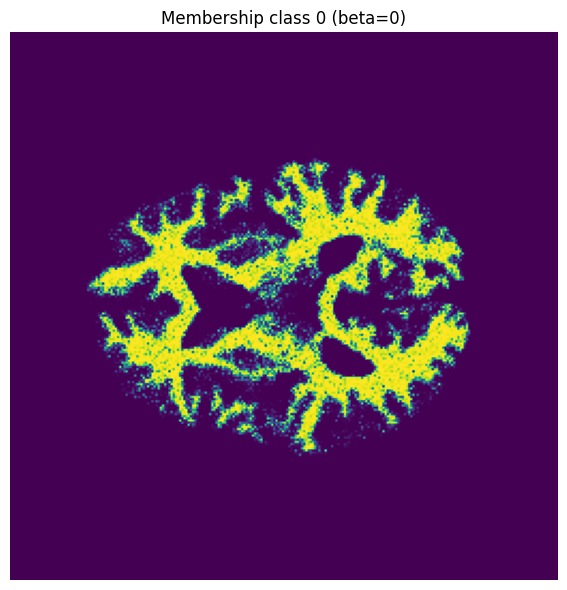
\includegraphics[width=0.3\textwidth]{Q2_membership_class_0_beta_0.png}
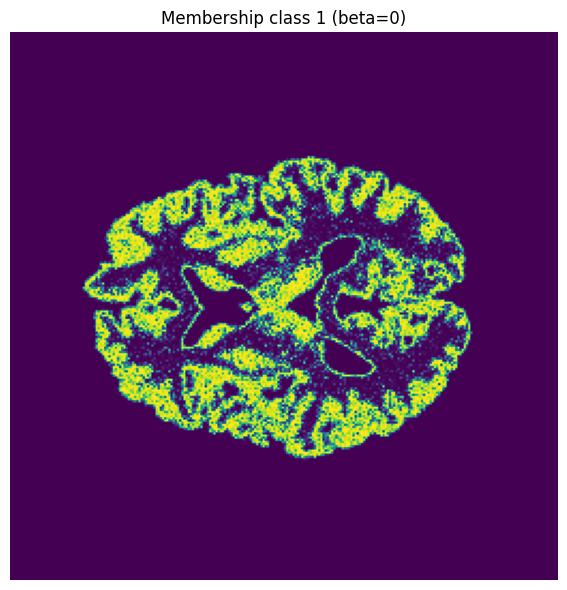
\includegraphics[width=0.3\textwidth]{Q2_membership_class_1_beta_0.png}
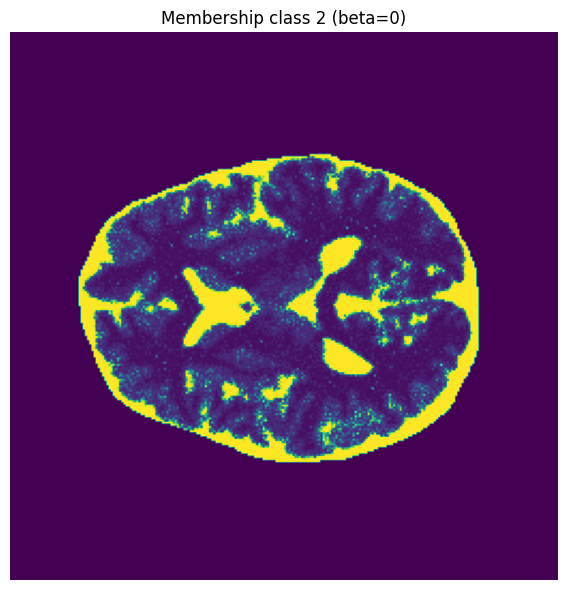
\includegraphics[width=0.3\textwidth]{Q2_membership_class_2_beta_0.png}
\caption{Membership maps for the three classes.}
\end{figure}


\subsection{Estimated Parameters}

Final estimated means for $\beta = 1.0$:

\[
\mu = [0.632, 0.521, 0.298]
\]

Final standard deviations for $\beta = 1.0$:

\[
\sigma = [0.0014, 0.0016, 0.0084]
\]

Final estimated means for $\beta = 0.0$:

\[
\mu = [0.64, 0.535, 0.38]
\]

Final standard deviations for $\beta = 0.0$:

\[
\sigma = [0.0012, 0.0015, 0.0185]
\]

\subsection{Effect of MRF Prior}

Comparison between $\beta = 1.0$ and $\beta = 0$ shows:

\begin{itemize}
\item MRF reduces noise in segmentation
\item Regions become spatially smoother
\item Boundaries are more coherent
\end{itemize}

Without MRF, segmentation is noisy and fragmented.


\subsection{Conclusion}

The EM-GMM framework with MRF prior successfully segments the brain MRI. The mean-field approximation and ICM updates ensure efficient optimization, while the MRF prior significantly improves spatial consistency compared to standard EM without spatial modeling.
\end{document}